\documentclass{amsart}
\pdfminorversion=7 
\usepackage{amssymb}
\renewcommand{\baselinestretch}{1.5}
\addtolength{\textwidth}{.2in}
\addtolength{\topmargin}{-.5in}
\addtolength{\textheight}{1in}

\usepackage{ifthen}
\usepackage{graphicx}
\usepackage{color}


\newlength{\cwidth}
\newcommand{\cents}{\settowidth{\cwidth}{c}%
\divide\cwidth by2
\advance\cwidth by-.1pt
c\kern-\cwidth
\vrule width .1pt depth.2ex height1.2ex
\kern\cwidth}

\newcommand{\sageprompt}{ {\tt sage$>$} }
\newcommand{\tab}{\rule{20pt}{0pt}}
\newcommand{\blnk}{\rule{1.5pt}{0pt}\rule{.4pt}{1.2pt}\rule{9pt}{.4pt}\rule{.4pt}{1.2pt}\rule{1.5pt}{0pt}}
\newcommand{\suchthat}{\; \rule[-3pt]{.25pt}{13pt} \;}
\newcommand{\divides}{\!\mid\!}
\newcommand{\tdiv}{\; \mbox{div} \;}
\newcommand{\restrict}[2]{#1 \,\rule[-4pt]{.125pt}{14pt}_{\,#2}}
\newcommand{\lcm}[2]{\mbox{lcm} (#1, #2)}
\renewcommand{\gcd}[2]{\mbox{gcd} (#1, #2)}
\newcommand{\Naturals}{{\mathbb N}}
\newcommand{\Integers}{{\mathbb Z}}
\newcommand{\Znoneg}{{\mathbb Z}^{\mbox{\tiny noneg}}}
\newcommand{\Enoneg}{{\mathbb E}^{\mbox{\tiny noneg}}}
\newcommand{\Qnoneg}{{\mathbb Q}^{\mbox{\tiny noneg}}}
\newcommand{\Rnoneg}{{\mathbb R}^{\mbox{\tiny noneg}}}
\newcommand{\Rationals}{{\mathbb Q}}
\newcommand{\Reals}{{\mathbb R}}
\newcommand{\Complexes}{{\mathbb C}}
%\newcommand{\F2}{{\mathbb F}_{2}}
\newcommand{\relQ}{\mbox{\textsf Q}}
\newcommand{\relR}{\mbox{\textsf R}}
\newcommand{\nrelR}{\mbox{\raisebox{1pt}{$\not$}\rule{1pt}{0pt}{\textsf R}}}
\newcommand{\relS}{\mbox{\textsf S}}
\newcommand{\relA}{\mbox{\textsf A}}
\newcommand{\Dom}[1]{\mbox{Dom}(#1)}
\newcommand{\Cod}[1]{\mbox{Cod}(#1)}
\newcommand{\Rng}[1]{\mbox{Rng}(#1)}

\DeclareMathOperator\caret{\raisebox{1ex}{$\scriptstyle\wedge$}}

\newtheorem*{defi}{Definition}
\newtheorem*{exer}{Exercise}
\newtheorem{thm}{Theorem}[section]
\newtheorem*{thm*}{Theorem}
\newtheorem{lem}[thm]{Lemma}
\newtheorem{cor}{Corollary}
\newtheorem{conj}{Conjecture}

\renewenvironment{proof}%
{\begin{quote} \emph{Proof:} }%
{\rule{0pt}{0pt} \newline \rule{0pt}{15pt} \hfill Q.E.D. \end{quote}}


\addtolength{\abovedisplayskip}{0pt}
\addtolength{\belowdisplayskip}{24pt}
\addtolength{\abovedisplayshortskip}{0pt}
\addtolength{\belowdisplayshortskip}{48pt}
\newcommand{\vsp}{\rule[-12pt]{0pt}{48pt}}

\begin{document}
\thispagestyle{empty}

\centerline{\Large Activity 31 -- Introduction to Proof}
\centerline{\large equivalence relations}

\bigskip
\Large


\begin{enumerate}
	
\item (Exercise 1 in GIAM section 6.3) Consider the relation $\relA$ defined by 
\[ \relA = \{ (x,y) \suchthat \; x \, \mbox{has the same astrological sign as} \, y \}. \]


Verify that $\relA$ is reflexive, symmetric, and transitive.

\vfill

\vfill

\newpage

\item Consider the generic ``equivalence mod $m$'' relation:

\[ x \relR y \quad \iff \quad x \mod{m} \; = \; y \mod{m} . \]

Show that $\relR$ is reflexive, symmetric and transitive.  

\vfill

\newpage


\item In the book we defined the function $sf(n)$ which returns $n$ divided by the largest perfect square that divides $n$.  For example $sf(20) = 5$ since $4$ is the largest perfect square that divides $20$, and $20/4 = 5$ 

Use the $sf$ function to define a relation:

\[ x \relS y \quad \iff \quad sf(x) = sf(y) \]

Show that $\relS$ is an equivalence relation on $\Naturals$.

\vfill 

\newpage

\item Continuing with the relation $\relS$ defined in problem 4, notice that for any number $x$ that actually is a perfect square, $sf(x) = 1$.  Given this, what is $\overline{1}$?

\vfill


\item (Still working with the relation from problem 4.)  Many different natural numbers can be used as a ``label'' for the equivalence classes under $\relS$.  For instance $\overline{2}$, $\overline{8}$ and $\overline{18}$ all denote the same equivalence class -- let's follow the convention of always using the smallest such label.  Characterize these reduced representatives for the equivalence classes.

\vfill

\newpage

\item Define a relation $\relQ$ on the set of all finite sets by

\[ A \relQ B \quad \iff \quad  |A| = |B| \]

What are the equivalence classes under $\relQ$?

\vfill

\item (Exercise 3 in GIAM section 6.3.)

Define a relation $\relA$ on the set of all words by

\[ w_1 \relA w_2 \quad \iff \quad w_1 \mbox{ is an anagram of } w_2. \]

\noindent Show that $\relA$ is an equivalence relation.  (Words are anagrams
if the letters of one can be re-arranged to form the other.  For example, `ART' and `RAT' are anagrams.)

\vfill

\newpage

\item (Exercise 4 in GIAM section 6.3.)

The two diagrams below both show a famous graph known as the 
\index{Petersen graph}Petersen graph.  The picture on the 
left is the usual representation which emphasizes its five-fold symmetry.  The picture on the right
highlights the fact that the Petersen graph also has a three-fold symmetry.  Label the right-hand diagram
using the same letters (A through J) in order to show that these two representations are truly isomorphic.

\vspace{.2in}

\rule{0pt}{0pt} \hspace{-.75in} \begin{picture}(0,0)%
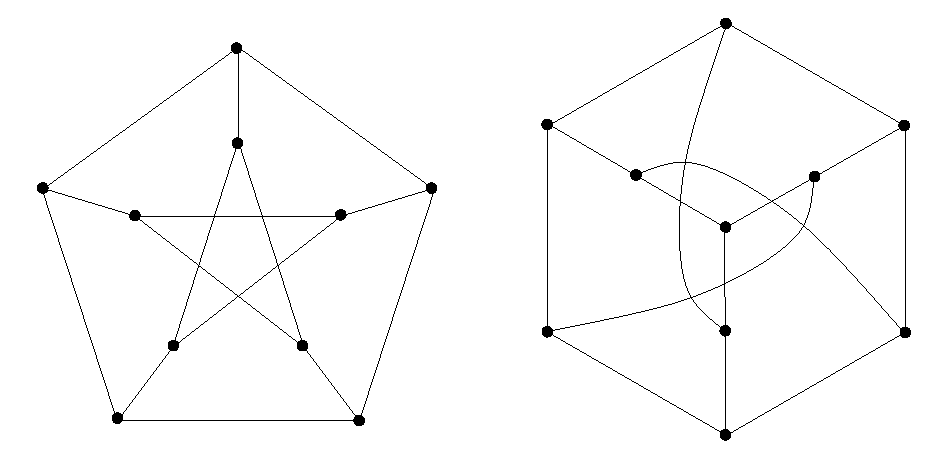
\includegraphics{./petersen_iso.eps}%
\end{picture}%
\setlength{\unitlength}{3947sp}%
\begin{picture}(7159,3450)(1453,-8445)
\put(2519,-7663){\makebox(0,0)[lb]{\smash{\fontsize{12}{14.4}\normalfont {I}%
}}}
\put(3280,-5177){\makebox(0,0)[lb]{\smash{\fontsize{12}{14.4}\normalfont {A}%
}}}
\put(4846,-6295){\makebox(0,0)[lb]{\smash{\fontsize{12}{14.4}\normalfont {B}%
}}}
\put(4231,-8422){\makebox(0,0)[lb]{\smash{\fontsize{12}{14.4}\normalfont {C}%
}}}
\put(2126,-8430){\makebox(0,0)[lb]{\smash{\fontsize{12}{14.4}\normalfont {D}%
}}}
\put(1468,-6280){\makebox(0,0)[lb]{\smash{\fontsize{12}{14.4}\normalfont {E}%
}}}
\put(3316,-5978){\makebox(0,0)[lb]{\smash{\fontsize{12}{14.4}\normalfont {F}%
}}}
\put(4116,-6756){\makebox(0,0)[lb]{\smash{\fontsize{12}{14.4}\normalfont {G}%
}}}
\put(3839,-7661){\makebox(0,0)[lb]{\smash{\fontsize{12}{14.4}\normalfont {H}%
}}}
\put(2244,-6796){\makebox(0,0)[lb]{\smash{\fontsize{12}{14.4}\normalfont {J}%
}}}
\end{picture}%


\vspace{.2in}

\vfill

\end{enumerate}


\end{document}
